\input{chapter-header.tex}
% ===========================================================================
\chapter{Implementing Object Spaces}
\minitoc
% ===========================================================================
\introduction
% ===========================================================================


% ===========================================================================
\section{One API, Several Backends}

% ===========================================================================
\section{The VM Backend: Several Object Spaces on the Same Virtual Machine}


We implemented Oz\footnote{The code can be found under \url{http://www.smalltalkhub.com/\#!/~Guille/ObjectSpace} with licence MIT} in the Pharo 2.0 platform. Our solution virtualizes Pharo images and provides, as already described, the ability to fully control their object graph, inject objects in a safe way and control their execution.

Our implementation includes a language side library resembling the membrane objects and an extension to the Stack virtual machine. We decided to extended the Stack virtual machine to avoid dealing with the complexity of the Just In Time (JIT) compiler. The virtual machine extensions, described in Sections \ref{sec:context_switch} and \ref{sec:object_space_creation}, include the addition of three primitives~(load an image into the object memory, transfer the execution to an \objectspace, and install an image in an \objectspace as host) and the modification of the function in charge of the context switch mechanism.

%Figure \ref{fig:objectSpaceImplementationOverview} shows a detailed overview of our solution.

%\begin{figure*}[!ht]
%\begin{center}
%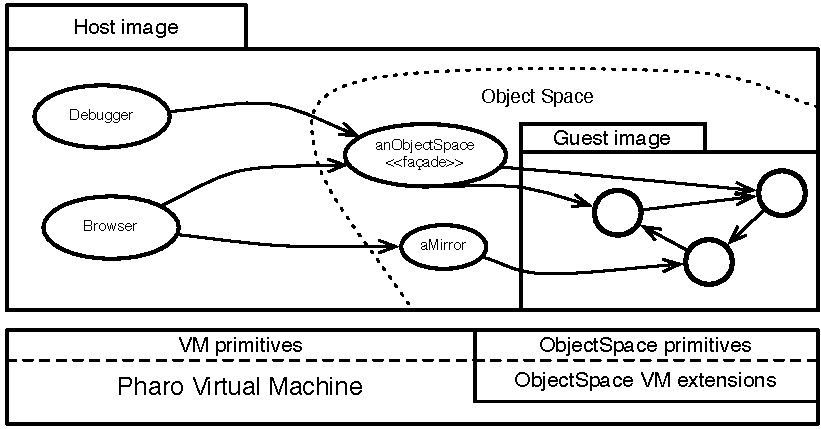
\includegraphics[width=.9\linewidth]{objectSpaceOverview}
%\caption{Object Spaces encapsulate a virtualized image\label{fig:objectSpaceImplementationOverview}}
%\end{center}
%\end{figure*}

In this section, we explain the details of our solution's implementation. We intend this section to document both the features a programming platform~(language and virtual machine) should provide to build this kind of solution and the way our solution uses those features.

\subsection{Related work to this implementation}
In the field of virtualizing reflective object oriented languages and their runtimes, we did not find so far a work directly related with our solution. There are, however, works on isolation related with some parts of it, specially with the internal low level implementation details.

The memory layout we implemented has, as we stated in sections \ref{sec:memory} and \ref{sec:not_yet_implemented}, many advantages regarding the development of our solution, but presents also many drawbacks. 
Sharing the object memory between different images implies that there is no need for special support on \emph{cross-image references}, and that the existing memory management in the virtual machine can be used transparently.
However, this solution forbids the host to analyze the \objectspace memory usage, and has an impact on the GC.

J-Kernel \cite{Hawb98a} and Luna \cite{Hawb02a} present a solution similar to ours regarding the memory usage. They are Java solution for isolating object graphs with security purposes. In them, each object graph is called a \emph{protection domain}. All protection domains loaded in a system, and their objects, share the same memory space. 

The J-Kernel enforces the separation between domains by using the Java type system, the inability of the Java language to forge object references, and by providing capability objects\cite{Levy84a,Mill03a,Spoo00a} enabling remote messaging and controlling the communication. This same separation in Luna \cite{Hawb02a} is achieved by the modification of the type system and the addition in the virtual machine of the \emph{remote reference} concept. In our solution, the separation is given by the same inability to forge object references and the membrane objects that control the communication.

KaffeOS \cite{Back00a} makes an explicit domain separation in memory by using different memory heaps in the virtual machine. They enforce domain separation by using memory write barriers. Cross-domain references become cross-heap references, and thus, they need special virtual machine support.

Regarding the threading model~(cf. Section \ref{sec:context_switch}), a Pharo virtual machine has single threaded execution. Only one operating system thread is used to execute Pharo code, so process scheduling is handled internally by the virtual machine. Processes scheduled using this approach are also called \emph{green threads}~\gp{cite green threads!!}. Green threads provide process scheduling without native operative system support while limiting the proper usage of modern multicore CPUs. In our implementation, their usage allowed us to reuse the current virtual machine scheduling. We also use a green thread approach to schedule image execution. All images are executed in the same single thread, one at a time. This model simplifies our implementation because it avoids concurrency problems between host and guest images.

KaffeOS presents a model where resource accounting is handled at the level of the virtual machine. Our solution aims to control and account resources at the language level. However, our implementation is not complete yet on this front.

Worlds~\cite{Wart08a} scope side-effects of Javascript programs by reifying the notion of its state. Our solution takes a similar approach by reifying images. In our solution, images have a notion of their own state just like Javascript Worlds, but include also its manipulation from the outside.



\subsection{Memory Layout} \label{sec:memory}

We decided to make an \objectspace share the same memory space~(the object memory) used by the host. Then, objects from both host and guest are mixed in the object memory, and not necessarily contiguous, as shown in Figure \ref{fig:heap}. This decision is funded on minimizing the changes made to the virtual machine, because of its complex state of the art. Our decision, while easing the development of our solution, has the following impact on it:

\begin{figure*}[htb]
\begin{center}
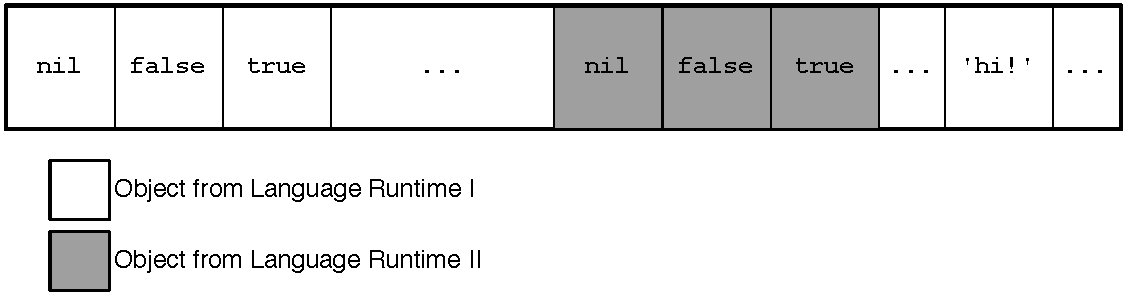
\includegraphics[width=.63\linewidth]{object_spaces_heap}
\caption{Objects from the host and guest are mixed in the object memory. In this figure, after the \ct{nil}, \ct{true} and \ct{false} host instances, follow the corresponding ones of the guest, which can in order be followed by objects of the host, like the string \textbf{`hi'}. \label{fig:heap}}
\end{center}
\end{figure*}

\begin{description}
	\item \textbf{Reuse memory handling mechanisms.} We use the same existing memory infrastructure as when no \objectspaces are used. Existing mechanisms for allocating objects or growing the object memory when a limit is reached can be reused transparently by our implementation. 
	\item \textbf{Simplify the object reference mechanism.} References from the membrane objects to the guest image objects are handled as simple object references. No extra support from the virtual machine was developed in this regard.
	\item \textbf{Shared garbage collection.} Since objects from the host and guest are mixed in the object memory, and their boundaries are not clear from the memory point of view, the garbage collector~(GC) is shared between them. Every GC run must iterate over all their objects, increasing its time to run.
	
	\item \textbf{Observer's effect on an \objectspace's memory.} Analyzing and controlling an \objectspace's memory still suffers from the \emph{observer's effect} in our solution: every action taken by the host on the \objectspace modifies the shared memory, and therefore alters the process. Because of this, an \objectspace's memory cannot be properly analyzed.
\end{description}

\subsection{Mirror Implementation}

Our implementation of mirrors manipulate the objects inside an \objectspace by using already existing primitives. There was no need to implement new primitives in the virtual machine since the existence of two primitives:
\begin{description}
	\item \textbf{Execute a given method on an object.} Given a method, it is possible to execute it on an object, avoiding method lookup in the object. In the current virtual machine, this primitive is implemented in the method \textbf{\ct{receiver:withArguments:executeMethod:}} of the \ct{CompiledMethod} class, with number 188. This method receives as arguments the object on which the primitive will be executed, an array of arguments, and the methods to execute.
	\item \textbf{Execute a primitive on an object.} It is possible to send a message to an object, so a primitive is executed on the receiver. This primitive is implemented in Pharo's \ct{ProtoObject} class as \textbf{\ct{tryPrimitive:withArgs:}} with number 118 and receives as argument the number of the primitive and an array or arguments.
\end{description}

Since the primitive \ct{tryPrimitive:withArgs:} executes the given primitive on the receiver of the message, and we want our mirrors to avoid \emph{cross image-message sends}~(cf. Section \ref{sec:model_mirrors}), we combine both primitives. We use primitive \ct{receiver:withArguments:executeMethod:} to execute the primitive method \ct{tryPrimitive:withArgs:} on the object from the guest image, avoiding the \emph{cross image-message send} and executing directly the primitive on the given object.

\begin{figure}[htb]
\begin{code}
CompiledMethod
       receiver: aGuestObject
       withArguments: \{ aPrimitiveNumber . anArrayOfArguments \}
       executeMethod: (ProtoObject >> #tryPrimitive:withArgs:)
\end{code}
\caption{Combining the two \emph{meta primitives} to execute a primitive on a guest object\label{code:meta_primitives}}
\end{figure}

Our mirror system contains three main mirrors regarding the internal representation of objects: a mirror for objects containing just object references such as \ct{Array} or \ct{OrderedCollection}, a mirror for objects with non-reference word fields such as \ct{Float} or \ct{WordArray} and a last one for objects with byte fields such as \ct{ByteArray} or \ct{ByteString}. In addition to them, we provide specialized mirrors for some kind of objects. The list of current mirrors we provide is the following: ObjectMirror, ByteObjectMirror, WordObjectMirror, ClassMirror, MetaclassMirror, ClassPoolMirror, MethodDictionaryMirror, MethodMirror, ContextMirror, ProcessSchedulerMirror and ProcessMirror.

\subsection{Process Manipulation and Scheduling}

Processes inside an \objectspace are exposed to the host image as mirrors. Resuming/activating a process consists in removing it from the suspended list in its scheduler and put it as the active process in its image. Suspend a process consists in putting the process in the corresponding suspension list of its process scheduler. The ProcessMirror and the ProcessSchedulerMirror handle the scheduling in the guest image and keep the consistency in the \objectspace process scheduler.

Using Oz, we can also create and install new processes inside an \objectspace given a code expression. The creation of a process requires the creation of a compiled method with the code~(bytecode) corresponding to the desired expression and a method context. The compiled method with the code to run is obtained by compiling the expression in the host and creating an \objectspace compiled method. The \objectspace compiled method is then provided with the compiled bytecode and its corresponding literals.

\subsection{Context Switch between Images} \label{sec:context_switch}

Pharo virtual machine holds the state of the image running into the \emph{special objects array} object. The special objects array is a simple array object referencing special objects directly accessed and used by the virtual machine. For example, it references objects such as the boolean and numeric classes or the \ct{nil}, \ct{true} and \ct{false} instances. Particularly, the special objects array contains a process scheduler object and its corresponding process objects, implementing green threads. Pharo virtual machine has a single threaded nature and uses green threads to organize its execution.

An \objectspace has its own special objects array, and thus, the code execution inside the \objectspace must use its special objects and not the ones in the host. We modified the virtual machine to be able to perform a context switch between the host and the \objectspace, and making it sensitive to the corresponding special objects array. We kept the single threaded nature of the vm, so the context switch between images puts the running image to sleep and awakens the new one. There are no concurrency problems between the different images.

Our modified VM has a special reference to the host's special objects array. To let an \objectspace run, we implemented a primitive to explicitly give control to the \objectspace by installing its special objects array. This primitive puts the current running process to sleep, changes the special objects array to the one request, and finally awakens the process installed as active in the \objectspace. Figure \ref{code:switch_to_objectspace} contains the VM code implementing this primitive.

\begin{figure}[htb]
\begin{code}
\textbf{primitiveResumeFromASpecialObjectsArray:}
                                                        aSpecialObjectsArray
    | oldProc activeContext  newProc |

    "we put to sleep the current running process"
    oldProcess := self activeProcess.
    statProcessSwitch := statProcessSwitch + 1.
    self push: instructionPointer.
    self externalWriteBackHeadFramePointers.
    activeContext := self
        ensureFrameIsMarried: framePointer
        SP: stackPointer.
    objectMemory
        storePointer: SuspendedContextIndex
        ofObject: oldProc
        withValue: activeContext.
	
    "we replace the special objects array"
    self replaceSpecialObjectsArrayWith: aSpecialObjectsArray.
	
    "we awake the process"
    newProc := self activeProcess.
    self externalSetStackPageAndPointersForSuspendedContextOfProcess: newProc.
    instructionPointer := self popStack

\textbf{replaceSpecialObjectsArrayWith:} newSpecialObjectsArray
    objectMemory specialObjectsOop: newSpecialObjectsArray.
    objectMemory nilObject:
             (objectMemory splObj: NilObject).
    objectMemory falseObject: 
             (objectMemory splObj: FalseObject).
    objectMemory trueObject:
             (objectMemory splObj: TrueObject).

    "Reinitialize VM state to point to the correct nil object"	
    method := objectMemory nilObject.
    messageSelector := objectMemory nilObject.
    newMethod := objectMemory nilObject.
    lkupClass := objectMemory nilObject.
\end{code}
\caption{VM functions written in Slang to transfer control to a virtualized image
\label{code:switch_to_objectspace}}
\end{figure}

Our implementation also supports the possibility to provide a controlled window of execution to an \objectspace. The current VM possesses a heartbeat thread it uses to provoke a context switch every 20 milliseconds. Our implementation uses the heartbeat mechanism to pause the current \objectspace process and give the control back to the host. We changed the VM function \textbf{\ct{checkForEventsMayContextSwitch:}} adding the code in Figure \ref{code:heartbeat_contextswitch}, to use the behavior implemented in the \ct{primitiveResumeFromASpecialObjectsArray:} primitive.

\begin{figure}[htb]
\begin{code}
((hostSpecialObjectArray ~~ objectMemory nilObject)
    and:
[objectMemory specialObjectsOop ~~ hostSpecialObjectArray])
        ifTrue: [ 
            self primitiveResumeFromASpecialObjectsArray:
                       hostSpecialObjectArray.
        ].
\end{code}
\caption{Additions to VM function \textbf{\ct{checkForEventsMayContextSwith:}} written in Slang to give back control to the host image.
\label{code:heartbeat_contextswitch}}
\end{figure}

\subsection{Creating an \objectspace} \label{sec:object_space_creation}

An \objectspace can be created either from scratch or by loading an existing image. Loading an existing image was implemented as a virtual machine primitive, because the image snapshot is actually a memory snapshot and therefore, easier to handle at VM level. This primitive, implemented with the code shown in Figure~\ref{code:import_image}, reads the snapshot file, puts all objects into the object memory, updates the object references to make them coherent and finally returns the special objects array of the loaded image.

\begin{figure}[htb]
\begin{code}
\textbf{primitiveLoadImage}
    | headerlength bytesRead newImageStart rootOffset oldBaseAddress dataSize rootOop fileObject |
    
    "get the reference to the file object"
    fileObject := self stackValue: 0.

    "Where will we put the new objects"
    newImageStart := objectMemory startOfFreeSpace.

    "read image header"
    self readLongFrom: fileObject.
    headerlength := self readLongFrom: fileObject.
    dataSize := self readLongFrom: fileObject.
    oldBaseAddress := self readLongFrom: fileObject.
    rootOffset :=
          (self readLongFrom: fileObject) - oldBaseAddress.
    
    "seek into the file the start of the objects"
    self seek: headerlength onFile: fileObject.
    
    "grow the heap in the ammount of the image size"
    objectMemory growObjectMemory: dataSize.
    
    "read the file into the free part of the memory"
    bytesRead := self
                    fromFile: fileObject
                    Read: dataSize
                    Into: newImageStart.

    "tell the vm the free space is now after the loaded objects"
    objectMemory advanceFreeSpace: dataSize.
         
    "update the pointers of the loaded objects"
    self
          updatePointersForObjectsPreviouslyIn: oldBaseAddress
          from: newImageStart
          until: newImageStart + dataSize.
    
    "return the special objects array"
    rootOop := newImageStart + rootOffset.
    self pop: 2 thenPush: rootOop.
\end{code}
\caption{Implementation of primitive \textbf{\ct{primitiveLoadImage}} that loads an image snapshot into the object memory written in Slang
\label{code:import_image}}
\end{figure}

On the other side, creating an \objectspace from scratch can be implemented as a bootstrap of the system, following the process defined in \cite{Poli12a}. The \objectspace provides the \textbf{\ct{createObjectWithFormat:}} method to create an object respecting the given format but with an anonymous class, so we can consider it as a "classless" object. This method is used in the first stage of the bootstrap process, when no classes are available in the \objectspace image yet, to create the \ct{nil} instance~(cf. Figure~\ref{code:bootstrap_nil}) and the first classes~(cf. Figure~\ref{code:bootstrap_classes}). Later, when the classes are available, those objects are set their corresponding ones by using the \textbf{\ct{setClass:}} message.

\begin{figure}[htb]
\begin{code}
theNil := objectSpace createObjectWithFormat: nilFormat.
objectSpace nilObject: theNil.
\end{code}
\caption{Bootstrapping an \objectspace: Creating a "classless" nil when there are no classes
\label{code:bootstrap_nil}}
\end{figure}

\begin{figure}[htb]
\begin{code}
metaclassMirror := objectSpace
    createClassWithFormat: classFormat
    forInstancesOfFormat: metaclassFormat.
metaclassClassMirror := objectSpace
    createClassWithFormat: metaclassFormat
    forInstancesOfFormat: classFormat.
 
metaclassMirror             setClass: metaclassClassMirror.
metaclassClassMirror    setClass: metaclassMirror.
\end{code}
\caption{Bootstrapping an \objectspace: Creating "classless" Metaclass and Metaclass class  when there are still no classes
\label{code:bootstrap_classes}}
\end{figure}

\subsection{Image Contract and Membrane Configuration}

Section \ref{sec:model_contract} states the need for establishing a contract between an image and the \objectspace in order to build the \objectspace membrane. This contract has, in our understanding, two complementary parts: the services an image provides, and the format to access them.

\begin{description}
	\item \textbf{Image services.} In order for the host to manipulate the image inside an \objectspace, the guest image must provide the required services. Those services are exposed as objects to the host, and their availability is given by how reachable they are in the object graph. For example, to get the list of classes inside an \objectspace or to manipulate its processes, its system dictionary and its processor should, respectively, be reachable in the image's object graph.
		
	Given a Pharo image from the current distribution, the reachability is constrained by its special objects array.
	The special objects array is the only object directly accessible of an image, since an image file contains in its header an explicit reference to it. So far, we understand the objects served by an image are the ones in the special objects array, which we detail in appendix \ref{app:specialObjectsArray}.
	
	The special objects array contains references to many of the objects the membrane needs: \ct{nil}, \ct{true}, \ct{false}, the processor, the numeric classes, the System dictionary, the compact classes, and some but not all literal classes.
	However, some elements in the special objects array are not mandatory in Pharo. For example, the System Dictionary may not available and then, there is no easy way to find all classes in the system. %The only way could be to assume the form of the graph and traverse it in an ad-hoc way.
	
	The current special objects array in Pharo does not provide all necessary services. It has to be extended to support, for example, the recovery of process objects suspended because of an error. These processes currently are only referenced by graphical debuggers, and thus not easily reachable from the special objects array. 

%	When built from scratch, an \objectspace can be configured at the image creation time because of the availability of the information needed by the membrane.
		 
	\item \textbf{The image format.} Given an object in the guest image, its enclosing \objectspace requires its internal representation and format to manipulate it correctly. We mean by internal representation its size, its amount of variable and fixed slots, the kind of and size of those slots, and in some cases their meaning.
	
	First, the semantics associated to the special objects array and its contents should be provided. That is, what does each index of the array mean.
	
	Second, the guest image may differ from the host Pharo image. Then, the \objectspace needs to make a correlation between the literal classes inside both host and guest to transform instances from and to the \objectspace format. The classes subject to this correlation in our current implementation are \ct{ByteString}, \ct{ByteSymbol}, \ct{Array}, \ct{SmallInteger}, \ct{Character} and \ct{Association}. Such correlation is done by providing the corresponding transformation methods.
	
	Finally, some mirrors must manipulate the internal state of special objects, and thus they must know their internal structure. The membrane configuration must provide the meaning of the instance variables of such special objects \ie the ProcessSchedulerMirror needs the index of the activeProcess and processList, and the ClassMirror needs the index of the superclass, method dictionary and name instance variables.
\end{description}

\subsection{Non Implemented Aspects} \label{sec:not_yet_implemented}
 
 For the sake of completion, we document in this subsection the aspects that have not been yet implemented in our solution.
 
Our current implementation does not handle properly the release of resources such as files or network connections~(sockets). In Pharo, the finalization and release of such resources is made in the language side. Given the single-threaded nature of our solution, an image running can provoke the garbage collection of any object in the memory even if they belong to another image, since the object memory is shared by all images~(cf. Section \ref{sec:memory}). However, garbage collection only activates in the current implementation the finalization process that belongs to the running image. The finalization processes of other images are ignored. Then, resources may leak, since they can be garbage collected but not properly finalized and released.

Another yet not implemented aspect regarding resources are global limitations imposed by the virtual machine. For example, the virtual machine memory is accounted globally without distinguish the usage per image; the virtual machine network plugin accounts and limits the amount of open sockets in a global way. In this sense, an image can use resources indiscriminately and restricting their use to other images \ie if there is a total of 100 sockets and an image opens 70, the rest of the images in the system have to share the 30 left.  

% ===========================================================================
\section{The Simulator Backend: an Object Space on a Simulated Virtual Machine}

% ===========================================================================
\section{The Remote Backend: an Object Space on a remote Virtual Machine}

% ===========================================================================
\section{Conclusion and Summary}

% =============================================================================
\input{chapter-footer.tex}